\documentclass{beamer}

\usepackage[utf8x]{inputenc}
\usepackage{beamerthemeSzeged}
\usepackage{graphicx}
\usepackage[font={scriptsize,it}]{caption}
\captionsetup[figure]{labelformat=empty}
\usepackage{graphics, setspace}
\usepackage{subfigure}
\usepackage{epsfig}

\usefonttheme{professionalfonts} % using non standard fonts for beamer
\usefonttheme{serif} % default family is serif
%\usepackage{fontspec}
%\setmainfont{Liberation Serif}
%\input{psfig}

\title{Mechanical Processing in Internally Coupled Ears}
\author{Anupam Prasad Vedurmudi}
\begin{document}
\begin{frame}
 \titlepage
\end{frame}

\section{Introduction}
\subsection{Pressure Difference Receiving Ears}
\begin{frame}
 Intro
\end{frame}

\section{The Model}

\begin{frame}
\frametitle{Mouth Cavity}
% \begin{figure}[htl]
% \flushleft
% 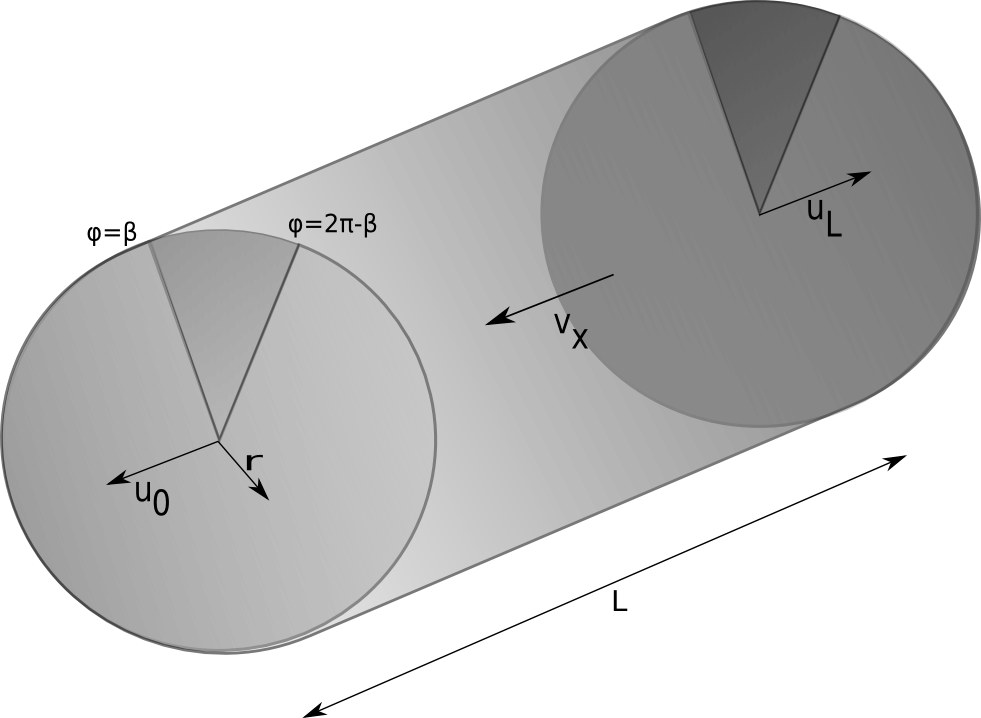
\includegraphics[width=.36\textwidth]{Diagrams/oldCylinder.png}
% %\caption{Previous Cylindrical Cavity}
% \end{figure}
\begin{figure}[htr]
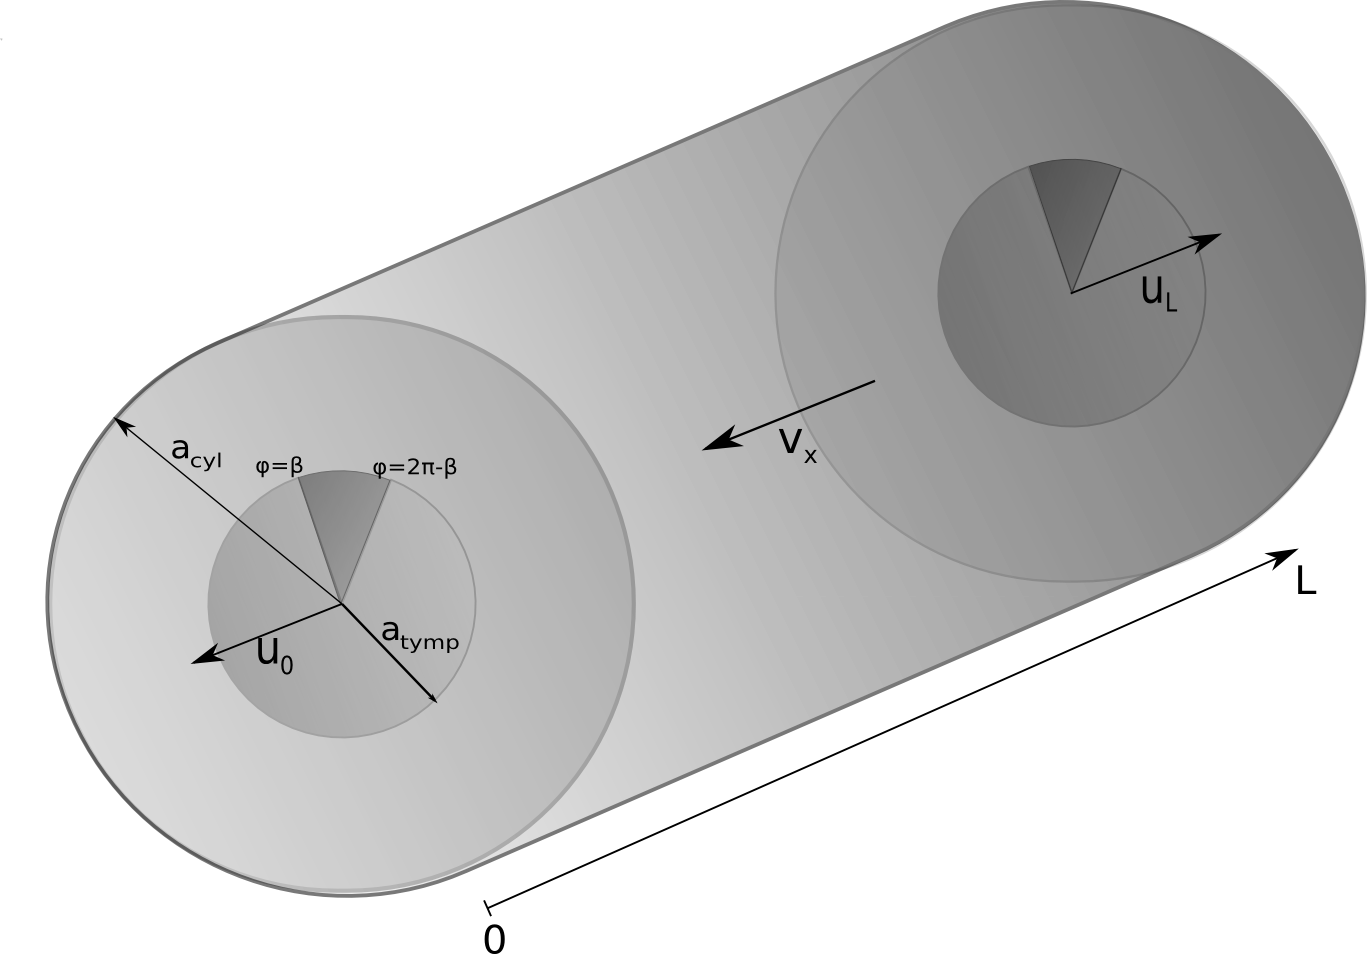
\includegraphics[width=.38\textwidth]{Diagrams/newCylinder.png}
\caption{Mouth Cavity Model}
\end{figure}

\end{frame}

\begin{frame}
\frametitle{Tympanum}
%  \begin{figure}[ht!]
%   \centering
%   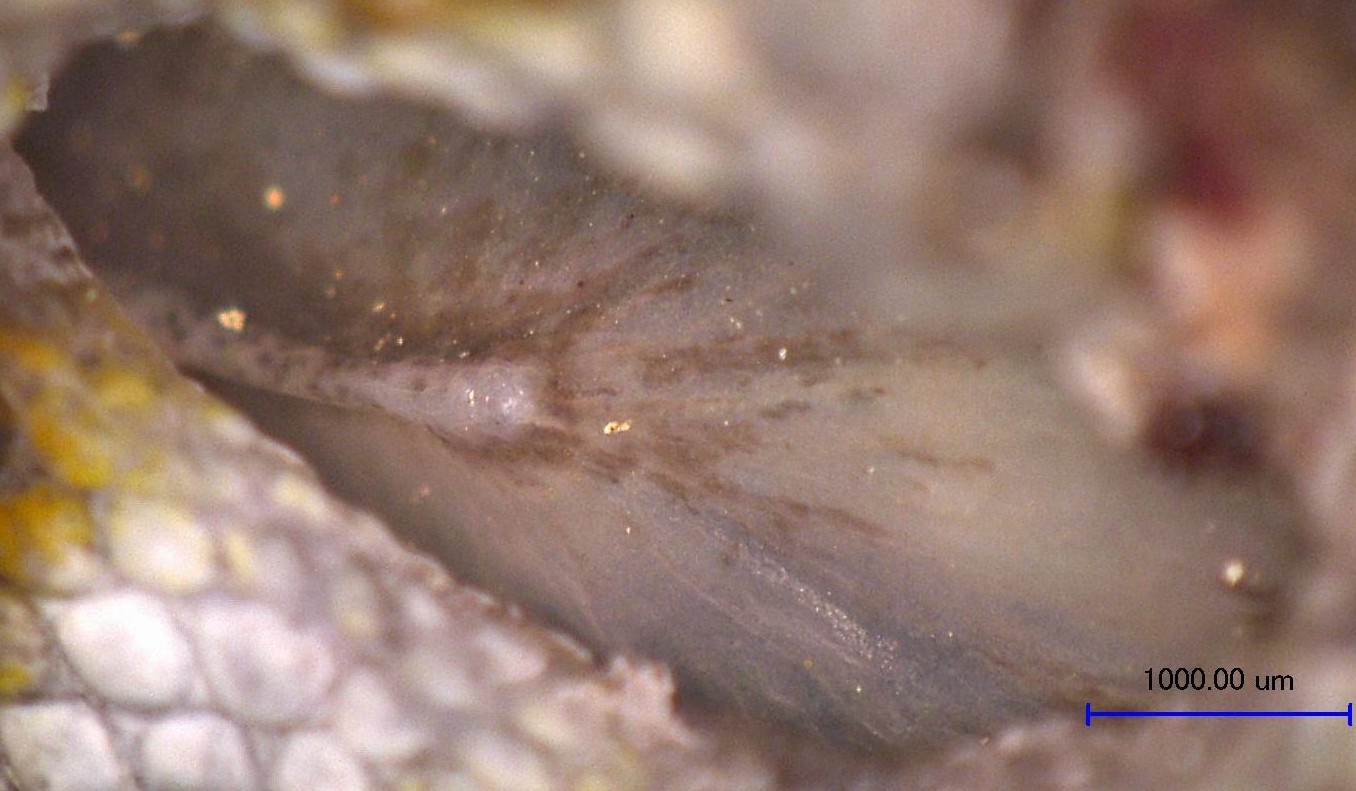
\includegraphics[width=.34\textwidth]{Diagrams/geckoextracolumella2.jpg}
% \end{figure}
\begin{figure}[htb!]
\makebox[\linewidth]{
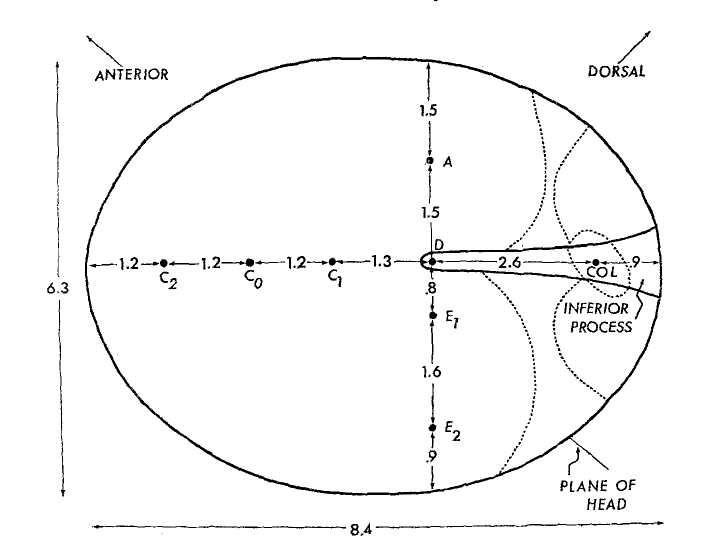
\includegraphics[width=.37\textwidth]{Diagrams/geckoear.png}
\hfill
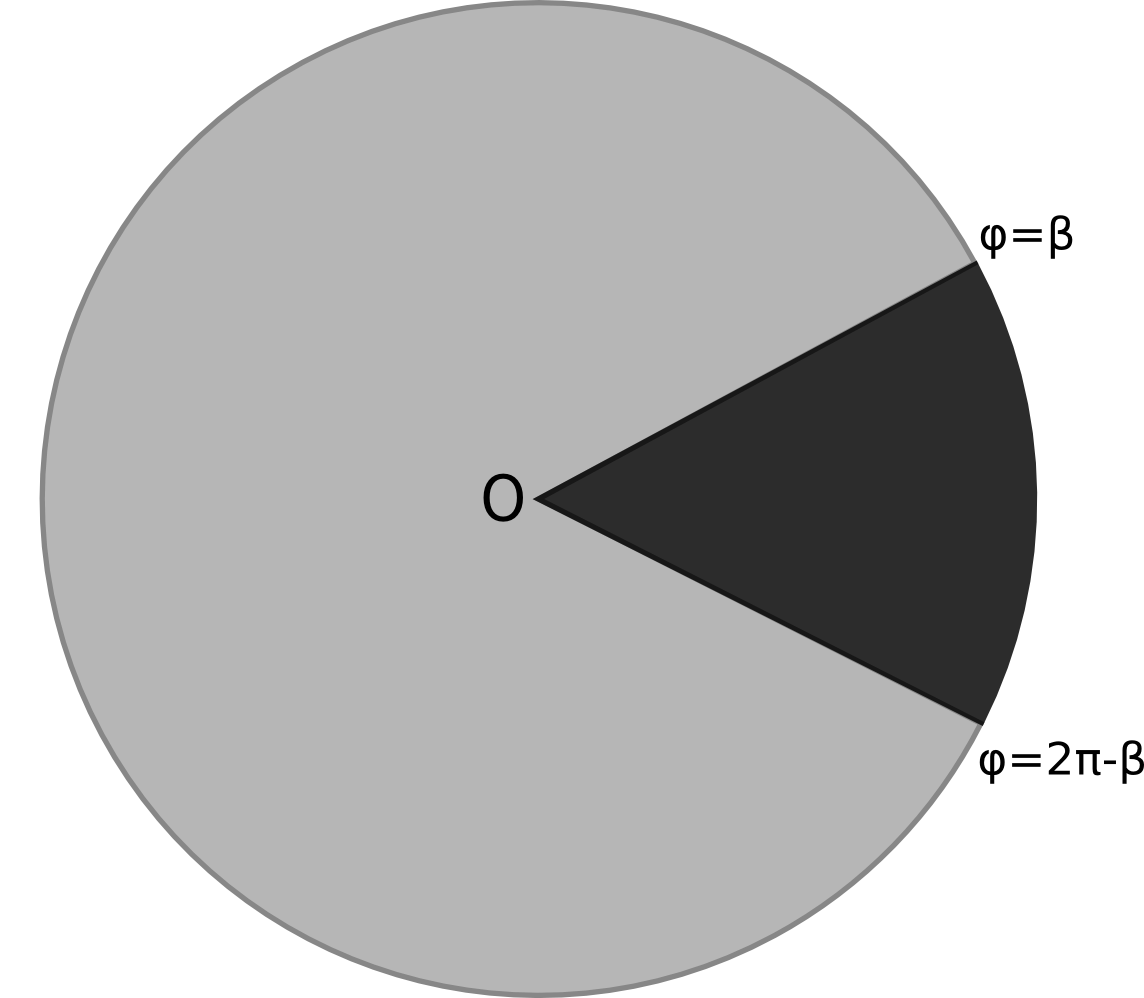
\includegraphics[width=.3\textwidth]{Diagrams/tympanummodel.png}}

\end{figure}

\end{frame}

\section{Evaluation}
\begin{frame}
 Evaluation
\end{frame}

\section{Conclusion}
\begin{frame}
 Conclusion
\end{frame}

\begin{frame}
 \frametitle{Thank You}
 \begin{figure}
  \centering
  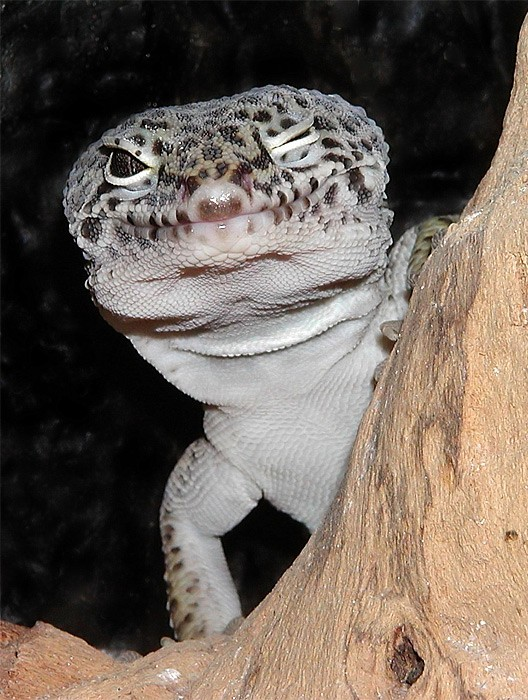
\includegraphics[width=.3\textwidth]{Diagrams/geckowink.jpg}
 \end{figure}

\end{frame}


\end{document}
